\documentclass[UTF8]{ctexart}
\usepackage{amsthm,amsmath,amsfonts,amssymb}
\usepackage{indentfirst,hyperref}
\usepackage{floatrow,graphicx,multicol,tcolorbox}
\usepackage{algorithm,algorithmicx,algpseudocode}
\usepackage{tikz}
\ctexset{section/format=\Large\bfseries}  % 参照讲义上的格式,标题左对齐
\usepackage[a4paper, hmargin=1.5cm, vmargin=2cm]{geometry}  % 页面大小和边距
\usepackage{enumitem}
\setlist{topsep=0pt,itemsep=-4pt}  % 列表间距
\pagestyle{plain}                  % ctex 默认的页码在右上角,改成下方
\setlength{\parskip}{0.5em}        % 段落间距
\title{基于字的三元模型的拼音输入法}
\author{熊泽恩~~计24}
\date{\today}
\hypersetup{
    colorlinks=true,
    linkcolor=black,
    urlcolor=blue,
    citecolor=blue
}

\begin{document}

\maketitle

\tableofcontents

\newpage

\section{拼音输入法}

\subsection{简介}

拼音输入法已经成了我们日常生活中不可分割的一部分。
为了简化问题,我们只考虑全拼,即每个汉字对应的拼音串是合法的、完整的汉语拼音。
现在的任务是,给定一个由全拼组成的拼音串,需要找到一个汉字串,
使得这个汉字串的拼音是给定的拼音串,同时该串在语料库中出现的概率最大。
概率越大,说明这个汉字串越有可能是用户想要输入的内容。

我们可以使用在《概率论与数理统计》这门课中学到的“条件概率”相关知识
来解决这个问题。

\subsection{输入输出格式}

\begin{itemize}
    \item 输入数据由多行拼音串构成,每行一个拼音串。
            拼音串中每个拼音之间用空格隔开。不含标点符号、阿拉伯数字等内容。
    \item 输出数据由多行汉字串构成,每行一个汉字串。
            汉字串中每个汉字之间没有空格。
\end{itemize}

\begin{table}[H]
    \centering
    \begin{tabular}{||l||l||}
        \hline
        输入(\texttt{input.txt}) & 输出(\texttt{output.txt}) \\
        \hline
        \texttt{gai lv lun yu shu li tong ji} & \em{概率论与数理统计} \qquad\qquad\qquad\qquad \\
        \texttt{pin yin shu ru fa} & \em{拼音输入法} \\
        \texttt{zhe shi yi ge ce shi} & \em{这是一个测试} \\
        \texttt{ni hao ma} & \em{你好吗} \\
        \hline
    \end{tabular}
    \caption{样例输入输出}
\end{table}

\section{基于字的三元模型}

\subsection{基本思路}

设 $\mathcal{F}$ 为所有合法拼音构成的集合,$\mathcal{G}$ 为所有合法汉字构成的集合。
从合法拼音的集合到合法汉字的集合的映射关系为 $\sigma: \mathcal{F} \to 2^{\mathcal{G}}$,
其中 $2^\mathcal{G}$ 表示 $\mathcal{G}$ 的幂集。
$\sigma$ 表示了一个拼音对应的所有可能的汉字。

对于一个由 $n$ 个拼音构成的序列 $S=s_1s_2\cdots s_n$,
我们需要需要确定每个单字拼音 $s_i$ 对应的中文字符 $w_i$,
使得中文序列 $w_1w_2\cdots w_n$ 最佳。给定 $S=s_1s_2\cdots s_n$,
我们定义 $P(w_1w_2\cdots w_n)$ 为
$w_1w_2\cdots w_n$ 与 $S$ 的匹配概率。

形式化地,我们需要找到一个 $W=w_1w_2\cdots w_n$,满足
$w_i \in \sigma(s_i), \forall i \in\{1, 2, \cdots, n\}$,
使得
\begin{equation*}
    P(w_1w_2\cdots w_n)
\end{equation*}
最大。

\subsection{公式推导}

根据条件概率的定义,我们有
\begin{align*}
\ln P(w_1 w_2 ... w_{n}) & = \ln P(w_1) + \ln P(w_2 \mid  w_1) + \ln P(w_3 \mid  w_1 w_2)
        + \cdots + \ln P(w_n \mid  w_1 w_2 \cdots w_{n-1}) \\
& = \sum_{i = 1}^{n}\ln P(w_i \mid  w_1w_2\cdots w_{i-1}). \tag{1}
\end{align*}

这一结果也是很容易理解的:我们可以将 $w_1w_2\cdots w_n$ 看作是一个序列,
找到最佳的 $w_i$ 的过程即为“汉字接龙”的过程,在给定 $w_1w_2\cdots w_{i-1}$
的条件下,我们需要找到一个 $w_i$ 使得 $w_1w_2\cdots w_i$ 的匹配概率最大。
例如,输入数据为 \texttt{dong wu yuan},我们已经得到 $\kaishu w_1 = \text{动}, w_2 = \text{物}$,
在这个条件下,我们需要找到 $w_3 \in \sigma(\texttt{yuan})$ 使得
$P(\kaishu\text{动物}\mid w_3)$ 最大。由于$\kaishu\text{园}$能使该概率最大
,因此最合理的选择。

在基于字的 $m$ 元模型中,我们认为在长度为 $m$ 的汉字串中,$w_i$ 仅仅与前 $m - 1$ 个汉字有关。
因此,我们可以将上述公式进一步简化为
\begin{equation*}
    \sum_{i = 1}^{n}\ln P(w_i\mid w_{i-m+1}\cdots w_{i-1}),
\end{equation*}
当 $m = 3$ 时,即为基于字的三元模型,我们需要最大化 $\sum_{i = 1}^{n}\ln P(w_i\mid w_{i-2}w_{i-1})$,
或者等价地,求
\begin{equation*}
    \sum_{i = 1}^{n}(-\ln P(w_i\mid w_{i-2}w_{i-1}))
\end{equation*}
的最小值。

由条件概率公式,对于每一项而言,有
\begin{equation*}
    P(w_i \mid  w_{i-2}w_{i-1}) = \dfrac{P(w_{i-2}w_{i-1}w_i)}{P(w_{i-2}w_{i-1})}.
\end{equation*}
再根据极大似然的思想,由于数据量足够大,所以可以用频次之比来估计概率之比。所以,上式可以近似为
\begin{equation*}
    P(w_i \mid  w_{i-2}w_{i-1}) \approx \dfrac{n(w_{i-2}w_{i-1}w_i)}{n(w_{i-2}w_{i-1})},
\end{equation*}
其中 $n(\cdot)$ 表示该汉字串在数据中的出现次数。

\subsection{图论建模}

我们可以将上述问题建模为一个有向无环图(Directed Acyclic Graph, DAG),如下所示:

\begin{figure}[htb!]
    \centering
    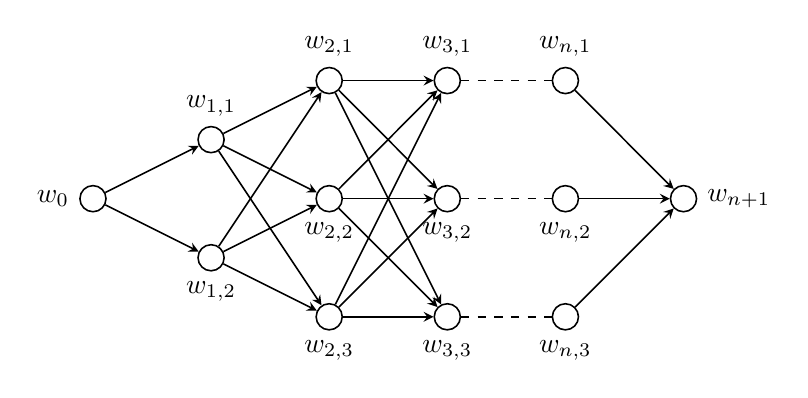
\begin{tikzpicture}[line width=.2mm,>=stealth]
        \pgfmathsetmacro{\h}{1.5}
        \pgfmathsetmacro{\w}{1.5}

        \node[draw,circle,label=left:{$w_0$}] (S) at (0,\h) {};

        \node[draw,circle,label=above:{$w_{1,1}$}] (W_11) at (\w,\h * 1.5) {};
        \node[draw,circle,label=below:{$w_{1,2}$}] (W_12) at (\w,\h * 0.5) {};

        \node[draw,circle,label=above:{$w_{2,1}$}] (W_21) at (\w * 2,\h * 2) {};
        \node[draw,circle,label=below:{$w_{2,2}$}] (W_22) at (\w * 2,\h) {};
        \node[draw,circle,label=below:{$w_{2,3}$}] (W_23) at (\w * 2,0) {};

        \node[draw,circle,label=above:{$w_{3,1}$}] (W_31) at (\w * 3,\h * 2) {};
        \node[draw,circle,label=below:{$w_{3,2}$}] (W_32) at (\w * 3,\h) {};
        \node[draw,circle,label=below:{$w_{3,3}$}] (W_33) at (\w * 3,0) {};

        \node[draw,circle,label=above:{$w_{n,1}$}] (W_n1) at (\w * 4,\h * 2) {};
        \node[draw,circle,label=below:{$w_{n,2}$}] (W_n2) at (\w * 4,\h) {};
        \node[draw,circle,label=below:{$w_{n,3}$}] (W_n3) at (\w * 4,0) {};

        \node[draw,circle,label=right:{$w_{n+1}$}] (T) at (\w * 5,\h) {};
        
        \draw[->] (S) -- (W_11);
        \draw[->] (S) -- (W_12);
        \draw[->] (W_11) -- (W_21);
        \draw[->] (W_11) -- (W_22);
        \draw[->] (W_11) -- (W_23);
        \draw[->] (W_12) -- (W_21);
        \draw[->] (W_12) -- (W_22);
        \draw[->] (W_12) -- (W_23);
        \draw[->] (W_21) -- (W_31);
        \draw[->] (W_21) -- (W_32);
        \draw[->] (W_21) -- (W_33);
        \draw[->] (W_22) -- (W_31);
        \draw[->] (W_22) -- (W_32);
        \draw[->] (W_22) -- (W_33);
        \draw[->] (W_23) -- (W_31);
        \draw[->] (W_23) -- (W_32);
        \draw[->] (W_23) -- (W_33);
        \draw[dashed] (W_31) -- (W_n1);
        \draw[dashed] (W_32) -- (W_n2);
        \draw[dashed] (W_33) -- (W_n3);
        \draw[->] (W_n1) -- (T);
        \draw[->] (W_n2) -- (T);
        \draw[->] (W_n3) -- (T);

    \end{tikzpicture}
    \caption{有向无环图}
\end{figure}

建图如下:其中 $w_0$ 为虚拟源点,$w_{n+1}$ 为虚拟汇点。
给 $\sigma(\cdot)$ 中的元素排序,
记 $w_{i, j}$ 为拼音 $s_i \in \mathcal{F}$ 所对应的第 $j$ 个汉字。
则 $w_{i-1, k}$ 与 $w_{i, j}$ 之间的边权满足
\begin{equation*}
\text{cost}(w_{i-1, k}, w_{i, j}) =
    \begin{cases}
        -\ln(P(w_{i, j})), & \text{if } i = 1, \\
        -\ln(P(w_{i, j}\mid w_{i-1, k})), & \text{if } i = 2, \\
        \min\limits_{v \in \sigma(s_{i-2})}(-\ln(P(w_{i, j}\mid v \; w_{i-1, k})), & \text{if } 3 \le i \le n, \\
        0, & \text{if } i=n+1.
    \end{cases}
\end{equation*}
这样我们得到了一个有向无环图。题目所求即为 $w_0$ 到 $w_{n+1}$ 的路径最小值。

\subsection{动态规划求解}

DAG 上最短路可以使用动态规划的思想来解决。设 $f(i, j)$ 表示从 $w_0$ 开始,到达 $w_{i, \cdot}$ 这一层对应的 $w_{i, j}$ 所需边权和的最小值。
则对于某一点 $w_{i, j}$ 而言,可以枚举它从上一层的哪一个点 $w_{i-1, k}$ 转移过来,
即可得到状态转移方程:
\begin{equation*}
f(i, j) = \max_{k \le \left|\sigma(s_{i - 1})\right|}(f(i - 1, k) + \text{cost}(w_{i-1, k}, w_{i, j})).
\end{equation*}
题目所求的 $w_0$ 到 $w_{n+1}$ 的路径最小值,即为 $f(n+1, w_{n+1})$。

\section{实验结果}

定义字准确率 $p_1$ 为
\begin{equation*}
    p_1 = \frac{\text{汉字正确个数}}{\text{总字数}},
\end{equation*}
句准确率 $p_2$ 为
\begin{equation*}
    p_2 = \frac{\text{所有汉字均正确的句子个数}}{\text{总句数}}.
\end{equation*}

除了三元模型以外,我还实现了模型更为简单的二元模型,即 $w_i$ 的选择仅与 $w_{i-1}$ 有关;
最终得到实验结果如下表所示:
\begin{table}[H]
    \centering
    \begin{tabular}{||c||c|c||}
        \hline
        评价指标 & 二元模型 & 三元模型 \\
        \hline
        句准确率 & $38.92\%$ & $46.51\%$ \\
        字准确率 & $83.72\%$ & $87.53\%$ \\
        平均单次响应时长 & $0.0135\;\mathrm{s}$ & $0.5909\;\mathrm{s}$ \\
        总响应时长 & $6.801\;\mathrm{s}$ & $296.1\;\mathrm{s}$ \\
        \hline
    \end{tabular}
    \caption{在测试集上的实验效果}
\end{table}
实验效果较为理想。由于三元模型比二元模型复杂,所以对应的两种准确率均更高;
而模型的复杂性也会导致所用计算时间更长,使得响应时长更长。
具体代码和实验数据已上传并开源于 \url{https://github.com/LeverImmy/Probability-and-Statistics-Thesis}。

\section{总结}

总而言之,我使用条件概率的方法,将拼音输入法问题建模为一个有向无环图上的最短路问题,
通过使用和极大似然的思想,将图上边权的计算简化为数据中的频次之比,
并最终使用动态规划的方法求解。

事实上,部分自然语言处理问题背后的原理与拼音输入法问题类似,本质上都是在已确定输出的前 $i$ 个 token
的情况下,预测第 $i+1$ 个 token 的概率分布,并输出概率最大的 token。

我觉得这个问题的解决方法比较有启发性,因为条件概率在《概率论与数理统计》
课程中是一个非常重要的概念;解决拼音输入法这个问题也很有意义,
因为拼音输入法是我们日常生活中不可或缺的一部分。
我通过利用课上学到的知识,将这两者结合起来,这让我感到非常有成就感。

\end{document}
